% Options for packages loaded elsewhere
\PassOptionsToPackage{unicode}{hyperref}
\PassOptionsToPackage{hyphens}{url}
\PassOptionsToPackage{dvipsnames,svgnames,x11names}{xcolor}
%
\documentclass[
]{article}

\usepackage{amsmath,amssymb}
\usepackage{iftex}
\ifPDFTeX
  \usepackage[T1]{fontenc}
  \usepackage[utf8]{inputenc}
  \usepackage{textcomp} % provide euro and other symbols
\else % if luatex or xetex
  \usepackage{unicode-math}
  \defaultfontfeatures{Scale=MatchLowercase}
  \defaultfontfeatures[\rmfamily]{Ligatures=TeX,Scale=1}
\fi
\usepackage{lmodern}
\ifPDFTeX\else  
    % xetex/luatex font selection
    \setmonofont[]{DejaVu Sans Mono}
\fi
% Use upquote if available, for straight quotes in verbatim environments
\IfFileExists{upquote.sty}{\usepackage{upquote}}{}
\IfFileExists{microtype.sty}{% use microtype if available
  \usepackage[]{microtype}
  \UseMicrotypeSet[protrusion]{basicmath} % disable protrusion for tt fonts
}{}
\makeatletter
\@ifundefined{KOMAClassName}{% if non-KOMA class
  \IfFileExists{parskip.sty}{%
    \usepackage{parskip}
  }{% else
    \setlength{\parindent}{0pt}
    \setlength{\parskip}{6pt plus 2pt minus 1pt}}
}{% if KOMA class
  \KOMAoptions{parskip=half}}
\makeatother
\usepackage{xcolor}
\setlength{\emergencystretch}{3em} % prevent overfull lines
\setcounter{secnumdepth}{5}
% Make \paragraph and \subparagraph free-standing
\makeatletter
\ifx\paragraph\undefined\else
  \let\oldparagraph\paragraph
  \renewcommand{\paragraph}{
    \@ifstar
      \xxxParagraphStar
      \xxxParagraphNoStar
  }
  \newcommand{\xxxParagraphStar}[1]{\oldparagraph*{#1}\mbox{}}
  \newcommand{\xxxParagraphNoStar}[1]{\oldparagraph{#1}\mbox{}}
\fi
\ifx\subparagraph\undefined\else
  \let\oldsubparagraph\subparagraph
  \renewcommand{\subparagraph}{
    \@ifstar
      \xxxSubParagraphStar
      \xxxSubParagraphNoStar
  }
  \newcommand{\xxxSubParagraphStar}[1]{\oldsubparagraph*{#1}\mbox{}}
  \newcommand{\xxxSubParagraphNoStar}[1]{\oldsubparagraph{#1}\mbox{}}
\fi
\makeatother

\usepackage{color}
\usepackage{fancyvrb}
\newcommand{\VerbBar}{|}
\newcommand{\VERB}{\Verb[commandchars=\\\{\}]}
\DefineVerbatimEnvironment{Highlighting}{Verbatim}{commandchars=\\\{\}}
% Add ',fontsize=\small' for more characters per line
\usepackage{framed}
\definecolor{shadecolor}{RGB}{241,243,245}
\newenvironment{Shaded}{\begin{snugshade}}{\end{snugshade}}
\newcommand{\AlertTok}[1]{\textcolor[rgb]{0.68,0.00,0.00}{#1}}
\newcommand{\AnnotationTok}[1]{\textcolor[rgb]{0.37,0.37,0.37}{#1}}
\newcommand{\AttributeTok}[1]{\textcolor[rgb]{0.40,0.45,0.13}{#1}}
\newcommand{\BaseNTok}[1]{\textcolor[rgb]{0.68,0.00,0.00}{#1}}
\newcommand{\BuiltInTok}[1]{\textcolor[rgb]{0.00,0.23,0.31}{#1}}
\newcommand{\CharTok}[1]{\textcolor[rgb]{0.13,0.47,0.30}{#1}}
\newcommand{\CommentTok}[1]{\textcolor[rgb]{0.37,0.37,0.37}{#1}}
\newcommand{\CommentVarTok}[1]{\textcolor[rgb]{0.37,0.37,0.37}{\textit{#1}}}
\newcommand{\ConstantTok}[1]{\textcolor[rgb]{0.56,0.35,0.01}{#1}}
\newcommand{\ControlFlowTok}[1]{\textcolor[rgb]{0.00,0.23,0.31}{\textbf{#1}}}
\newcommand{\DataTypeTok}[1]{\textcolor[rgb]{0.68,0.00,0.00}{#1}}
\newcommand{\DecValTok}[1]{\textcolor[rgb]{0.68,0.00,0.00}{#1}}
\newcommand{\DocumentationTok}[1]{\textcolor[rgb]{0.37,0.37,0.37}{\textit{#1}}}
\newcommand{\ErrorTok}[1]{\textcolor[rgb]{0.68,0.00,0.00}{#1}}
\newcommand{\ExtensionTok}[1]{\textcolor[rgb]{0.00,0.23,0.31}{#1}}
\newcommand{\FloatTok}[1]{\textcolor[rgb]{0.68,0.00,0.00}{#1}}
\newcommand{\FunctionTok}[1]{\textcolor[rgb]{0.28,0.35,0.67}{#1}}
\newcommand{\ImportTok}[1]{\textcolor[rgb]{0.00,0.46,0.62}{#1}}
\newcommand{\InformationTok}[1]{\textcolor[rgb]{0.37,0.37,0.37}{#1}}
\newcommand{\KeywordTok}[1]{\textcolor[rgb]{0.00,0.23,0.31}{\textbf{#1}}}
\newcommand{\NormalTok}[1]{\textcolor[rgb]{0.00,0.23,0.31}{#1}}
\newcommand{\OperatorTok}[1]{\textcolor[rgb]{0.37,0.37,0.37}{#1}}
\newcommand{\OtherTok}[1]{\textcolor[rgb]{0.00,0.23,0.31}{#1}}
\newcommand{\PreprocessorTok}[1]{\textcolor[rgb]{0.68,0.00,0.00}{#1}}
\newcommand{\RegionMarkerTok}[1]{\textcolor[rgb]{0.00,0.23,0.31}{#1}}
\newcommand{\SpecialCharTok}[1]{\textcolor[rgb]{0.37,0.37,0.37}{#1}}
\newcommand{\SpecialStringTok}[1]{\textcolor[rgb]{0.13,0.47,0.30}{#1}}
\newcommand{\StringTok}[1]{\textcolor[rgb]{0.13,0.47,0.30}{#1}}
\newcommand{\VariableTok}[1]{\textcolor[rgb]{0.07,0.07,0.07}{#1}}
\newcommand{\VerbatimStringTok}[1]{\textcolor[rgb]{0.13,0.47,0.30}{#1}}
\newcommand{\WarningTok}[1]{\textcolor[rgb]{0.37,0.37,0.37}{\textit{#1}}}

\providecommand{\tightlist}{%
  \setlength{\itemsep}{0pt}\setlength{\parskip}{0pt}}\usepackage{longtable,booktabs,array}
\usepackage{calc} % for calculating minipage widths
% Correct order of tables after \paragraph or \subparagraph
\usepackage{etoolbox}
\makeatletter
\patchcmd\longtable{\par}{\if@noskipsec\mbox{}\fi\par}{}{}
\makeatother
% Allow footnotes in longtable head/foot
\IfFileExists{footnotehyper.sty}{\usepackage{footnotehyper}}{\usepackage{footnote}}
\makesavenoteenv{longtable}
\usepackage{graphicx}
\makeatletter
\def\maxwidth{\ifdim\Gin@nat@width>\linewidth\linewidth\else\Gin@nat@width\fi}
\def\maxheight{\ifdim\Gin@nat@height>\textheight\textheight\else\Gin@nat@height\fi}
\makeatother
% Scale images if necessary, so that they will not overflow the page
% margins by default, and it is still possible to overwrite the defaults
% using explicit options in \includegraphics[width, height, ...]{}
\setkeys{Gin}{width=\maxwidth,height=\maxheight,keepaspectratio}
% Set default figure placement to htbp
\makeatletter
\def\fps@figure{htbp}
\makeatother

\usepackage{amsmath}
\usepackage{cancel}
\makeatletter
\@ifpackageloaded{caption}{}{\usepackage{caption}}
\AtBeginDocument{%
\ifdefined\contentsname
  \renewcommand*\contentsname{Table of contents}
\else
  \newcommand\contentsname{Table of contents}
\fi
\ifdefined\listfigurename
  \renewcommand*\listfigurename{List of Figures}
\else
  \newcommand\listfigurename{List of Figures}
\fi
\ifdefined\listtablename
  \renewcommand*\listtablename{List of Tables}
\else
  \newcommand\listtablename{List of Tables}
\fi
\ifdefined\figurename
  \renewcommand*\figurename{Figure}
\else
  \newcommand\figurename{Figure}
\fi
\ifdefined\tablename
  \renewcommand*\tablename{Table}
\else
  \newcommand\tablename{Table}
\fi
}
\@ifpackageloaded{float}{}{\usepackage{float}}
\floatstyle{ruled}
\@ifundefined{c@chapter}{\newfloat{codelisting}{h}{lop}}{\newfloat{codelisting}{h}{lop}[chapter]}
\floatname{codelisting}{Listing}
\newcommand*\listoflistings{\listof{codelisting}{List of Listings}}
\makeatother
\makeatletter
\makeatother
\makeatletter
\@ifpackageloaded{caption}{}{\usepackage{caption}}
\@ifpackageloaded{subcaption}{}{\usepackage{subcaption}}
\makeatother

\ifLuaTeX
  \usepackage{selnolig}  % disable illegal ligatures
\fi
\usepackage{bookmark}

\IfFileExists{xurl.sty}{\usepackage{xurl}}{} % add URL line breaks if available
\urlstyle{same} % disable monospaced font for URLs
\hypersetup{
  pdftitle={Homework 5},
  pdfauthor={Kevin Silberberg},
  colorlinks=true,
  linkcolor={blue},
  filecolor={Maroon},
  citecolor={Blue},
  urlcolor={Blue},
  pdfcreator={LaTeX via pandoc}}


\title{Homework 5}
\author{Kevin Silberberg}
\date{2024-11-14}

\begin{document}
\maketitle

\renewcommand*\contentsname{Table of contents}
{
\hypersetup{linkcolor=}
\setcounter{tocdepth}{3}
\tableofcontents
}

\section{Question 1}\label{question-1}

Consider a random variable \(\xi\) with PDF

\begin{equation}\tag{1}\label{pxi}
    p_{\xi}(x) = 
    \begin{cases}
        \frac{e^{-x}}{e - e^{-1}} & x \in [-1, 1] \\
        0 & \text{otherwise}
    \end{cases}
\end{equation}

see Figure~\ref{fig-pdfxi} for the plot of the PDF of \(\xi\).

\subsection{Part A}\label{part-a}

Use the Stieltjes algorithm to compute the sixth-order generalized
polynomial choas basis \[\{P_0(x), P_1(x), ..., P_6(x)\}\] for \(\xi\),
i.e.~a set of polynomials up to degree 6 that are orthogonal relative to
the PDF \(\xi\) given in \eqref{pxi}.

\subsubsection{Solution}\label{solution}

We know that since the distribution function \eqref{pxi} is compactly
supported, that the solution to the moment problem is unique and exists.

Let \(c = \frac{1}{e-e^{-1}}\) the constant in \(p_{\xi}(x)\)

Following the Stieltjes algorithm, let us compute the first orthogonal
polynomial and then we will write a code that computes the first six
orthogonal polynomials where \begin{align}
\mu(x) = ce^{-x}
\end{align}

is out weight function.

Let \(n = 0 \quad \pi_0 = 1 \quad \pi_{-1} = 0\)

\begin{align}
\alpha_0 &= \frac{\langle x , 1 \rangle}{\langle 1, 1 \rangle} \\
&= \frac{c \int_{-1}^{1}x e^{-x}dx}{c \int_{-1}^{1}e^{-x}dx} \\
&= \frac{\left[{-x e^{-x}}_{\bigg{\vert}_{-1}^{1}} - \int_{-1}^{1}-e^{-x}dx\right]}{\left[{-e^{-x}}_{\bigg{\vert}_{-1}^{1}}\right] } \\
&= \frac{-e^{-1} - e - e^{-1} + e}{-e^{-1} + e} \\
&= -\frac{2}{e^2 - 1} \approx -0.31304
\end{align}

Using \(\alpha_0\) let us find the first polynomial \(\pi_1\) using the
following formula

\begin{align}
\pi_{n+1}(x) = (x - \alpha_n)\pi_n(x) - \beta_n \pi_{n-1}(x)
\end{align}

\begin{align}
\pi_1(x) &= (x - \alpha_0)\pi_0 - \beta_0 \pi_{-1} \\
&= x + \frac{2}{e^2 - 1}
\end{align}

Let us now write a code that produces any arbitray number of orthogonal
polynomials with respect to the weight function.

\begin{Shaded}
\begin{Highlighting}[]
\ImportTok{using} \BuiltInTok{GLMakie}
\ImportTok{using} \BuiltInTok{QuadGK}
\ImportTok{using} \BuiltInTok{StaticArrays}

\CommentTok{\# weight function}
\FunctionTok{μ}\NormalTok{(x) }\OperatorTok{=} \FunctionTok{exp}\NormalTok{(}\OperatorTok{{-}}\NormalTok{x) }\OperatorTok{*} \OperatorTok{\^{}}\NormalTok{((}\FunctionTok{exp}\NormalTok{(}\FloatTok{1.0}\NormalTok{) }\OperatorTok{{-}} \OperatorTok{\^{}}\NormalTok{(}\FunctionTok{exp}\NormalTok{(}\FloatTok{1.0}\NormalTok{), }\OperatorTok{{-}}\FloatTok{1.0}\NormalTok{)), }\OperatorTok{{-}}\FloatTok{1.0}\NormalTok{)}

\CommentTok{\# define an integral using gauss{-}kronrod quadrature rule}
\FunctionTok{integ}\NormalTok{(x}\OperatorTok{::}\DataTypeTok{Function}\NormalTok{, sup}\OperatorTok{::}\DataTypeTok{SVector\{2\}}\NormalTok{) }\OperatorTok{=} \FunctionTok{quadgk}\NormalTok{(x, sup[}\FloatTok{1}\NormalTok{], sup[}\FloatTok{2}\NormalTok{]; atol}\OperatorTok{=}\FloatTok{1e{-}8}\NormalTok{, rtol}\OperatorTok{=}\FloatTok{1e{-}8}\NormalTok{)[}\FloatTok{1}\NormalTok{]}

\CommentTok{\# the support of the weight function}
\NormalTok{sup }\OperatorTok{=} \FunctionTok{SVector}\DataTypeTok{\{2\}}\NormalTok{(}\OperatorTok{{-}}\FloatTok{1.0}\NormalTok{, }\FloatTok{1.0}\NormalTok{)}

\KeywordTok{function} \FunctionTok{stieltjes}\NormalTok{(μ}\OperatorTok{::}\DataTypeTok{Function}\NormalTok{, N}\OperatorTok{::}\DataTypeTok{Int64}\NormalTok{, sup}\OperatorTok{::}\DataTypeTok{SVector\{2\}}\NormalTok{)}
    \CommentTok{\# μ: weight function defining the inner product}
    \CommentTok{\# N: number of orthogonal polynomials to compute}
    \CommentTok{\# sup: support (integration bounds) of the weight function}

\NormalTok{    M }\OperatorTok{=}\NormalTok{ N }\OperatorTok{+} \FloatTok{2}  \CommentTok{\# Extend size to accommodate buffer}
\NormalTok{    n }\OperatorTok{=} \FloatTok{2}      \CommentTok{\# Starting index for the recursion}

    \CommentTok{\# Initialize orthogonal polynomials (πn) as functions}
    \ConstantTok{π} \OperatorTok{=} \FunctionTok{Vector}\DataTypeTok{\{Function\}}\NormalTok{(}\ConstantTok{undef}\NormalTok{, M)}
    \ConstantTok{π}\NormalTok{[n}\OperatorTok{{-}}\FloatTok{1}\NormalTok{] }\OperatorTok{=}\NormalTok{ x }\OperatorTok{{-}\textgreater{}} \FloatTok{0.0} \OperatorTok{*}\NormalTok{ x}\OperatorTok{\^{}}\FloatTok{0.0}  \CommentTok{\# π₀(x) = 0}
    \ConstantTok{π}\NormalTok{[n] }\OperatorTok{=}\NormalTok{ x }\OperatorTok{{-}\textgreater{}} \FloatTok{1.0} \OperatorTok{*}\NormalTok{ x}\OperatorTok{\^{}}\FloatTok{0.0}    \CommentTok{\# π₁(x) = 1}

    \CommentTok{\# Initialize coefficient vectors αn and βn}
\NormalTok{    α }\OperatorTok{=} \FunctionTok{Vector}\DataTypeTok{\{Float64\}}\NormalTok{(}\ConstantTok{undef}\NormalTok{, M)}
\NormalTok{    β }\OperatorTok{=} \FunctionTok{Vector}\DataTypeTok{\{Float64\}}\NormalTok{(}\ConstantTok{undef}\NormalTok{, M)}
\NormalTok{    β[n}\OperatorTok{{-}}\FloatTok{1}\NormalTok{] }\OperatorTok{=} \FloatTok{0.0}  \CommentTok{\# β₀ = 0}
\NormalTok{    β[n] }\OperatorTok{=} \FloatTok{0.0}    \CommentTok{\# β₁ = 0}

    \CommentTok{\# Compute the first α coefficient (α₂)}
    \CommentTok{\# α₂ = ⟨xπ₁, π₁⟩ / ⟨π₁, π₁⟩}
\NormalTok{    α[n] }\OperatorTok{=} \FunctionTok{integ}\NormalTok{(x }\OperatorTok{{-}\textgreater{}}\NormalTok{ x }\OperatorTok{*} \ConstantTok{π}\NormalTok{[n](x) }\OperatorTok{*} \ConstantTok{π}\NormalTok{[n](x) }\OperatorTok{*} \FunctionTok{μ}\NormalTok{(x), sup) }\OperatorTok{/} \FunctionTok{integ}\NormalTok{(x }\OperatorTok{{-}\textgreater{}} \ConstantTok{π}\NormalTok{[n](x) }\OperatorTok{*} \ConstantTok{π}\NormalTok{[n](x) }\OperatorTok{*} \FunctionTok{μ}\NormalTok{(x), sup)}
    
    \CommentTok{\# Compute the next orthogonal polynomial π₂}
    \CommentTok{\# π₂(x) = (x {-} α₁)π₁(x) {-} β₁π₀(x)}
    \ConstantTok{π}\NormalTok{[n}\OperatorTok{+}\FloatTok{1}\NormalTok{] }\OperatorTok{=}\NormalTok{ x }\OperatorTok{{-}\textgreater{}}\NormalTok{ (x }\OperatorTok{{-}}\NormalTok{ α[n]) }\OperatorTok{*} \ConstantTok{π}\NormalTok{[n](x) }\OperatorTok{{-}}\NormalTok{ β[n] }\OperatorTok{*} \ConstantTok{π}\NormalTok{[n}\OperatorTok{{-}}\FloatTok{1}\NormalTok{](x)}

    \ControlFlowTok{for}\NormalTok{ n }\KeywordTok{in} \FloatTok{3}\OperatorTok{:}\NormalTok{M}\OperatorTok{{-}}\FloatTok{1}
\NormalTok{        α[n] }\OperatorTok{=} \FunctionTok{integ}\NormalTok{(x }\OperatorTok{{-}\textgreater{}}\NormalTok{ x }\OperatorTok{*} \ConstantTok{π}\NormalTok{[n](x) }\OperatorTok{*} \ConstantTok{π}\NormalTok{[n](x) }\OperatorTok{*} \FunctionTok{μ}\NormalTok{(x), sup) }\OperatorTok{/} \FunctionTok{integ}\NormalTok{(x }\OperatorTok{{-}\textgreater{}} \ConstantTok{π}\NormalTok{[n](x) }\OperatorTok{*} \ConstantTok{π}\NormalTok{[n](x) }\OperatorTok{*} \FunctionTok{μ}\NormalTok{(x), sup)}
\NormalTok{        β[n] }\OperatorTok{=} \FunctionTok{integ}\NormalTok{(x }\OperatorTok{{-}\textgreater{}} \ConstantTok{π}\NormalTok{[n](x) }\OperatorTok{*} \ConstantTok{π}\NormalTok{[n](x) }\OperatorTok{*} \FunctionTok{μ}\NormalTok{(x), sup) }\OperatorTok{/} \FunctionTok{integ}\NormalTok{(x }\OperatorTok{{-}\textgreater{}} \ConstantTok{π}\NormalTok{[n}\OperatorTok{{-}}\FloatTok{1}\NormalTok{](x) }\OperatorTok{*} \ConstantTok{π}\NormalTok{[n}\OperatorTok{{-}}\FloatTok{1}\NormalTok{](x) }\OperatorTok{*} \FunctionTok{μ}\NormalTok{(x), sup)}
        \ConstantTok{π}\NormalTok{[n}\OperatorTok{+}\FloatTok{1}\NormalTok{] }\OperatorTok{=} \ConstantTok{π}\NormalTok{[n}\OperatorTok{+}\FloatTok{1}\NormalTok{] }\OperatorTok{=}\NormalTok{ x }\OperatorTok{{-}\textgreater{}}\NormalTok{ (x }\OperatorTok{{-}}\NormalTok{ α[n]) }\OperatorTok{*} \ConstantTok{π}\NormalTok{[n](x) }\OperatorTok{{-}}\NormalTok{ β[n] }\OperatorTok{*} \ConstantTok{π}\NormalTok{[n}\OperatorTok{{-}}\FloatTok{1}\NormalTok{](x)}
    \ControlFlowTok{end}
    \ControlFlowTok{return} \ConstantTok{π}
\KeywordTok{end}
\ConstantTok{π} \OperatorTok{=} \FunctionTok{stieltjes}\NormalTok{(μ, }\FloatTok{6}\NormalTok{, sup)}
\end{Highlighting}
\end{Shaded}

Let us define a function that plots the first polynomial \(\pi_1(x)\)
over the numerical result as a validation.

\begin{Shaded}
\begin{Highlighting}[]
\KeywordTok{function} \FunctionTok{validatepione}\NormalTok{(}\ConstantTok{π}\OperatorTok{::}\DataTypeTok{Vector\{Function\}}\NormalTok{)}
    \FunctionTok{π\_1}\NormalTok{(x) }\OperatorTok{=}\NormalTok{ x }\OperatorTok{+}\NormalTok{ (}\FloatTok{2} \OperatorTok{/}\NormalTok{ (}\FunctionTok{exp}\NormalTok{(}\FloatTok{1}\NormalTok{)}\OperatorTok{\^{}}\FloatTok{2} \OperatorTok{{-}} \FloatTok{1}\NormalTok{))}
\NormalTok{    xs }\OperatorTok{=} \FunctionTok{LinRange}\NormalTok{(}\OperatorTok{{-}}\FloatTok{1}\NormalTok{, }\FloatTok{1}\NormalTok{, }\FloatTok{1000}\NormalTok{)}
\NormalTok{    fig }\OperatorTok{=} \FunctionTok{Figure}\NormalTok{()}
\NormalTok{    ax }\OperatorTok{=} \FunctionTok{Axis}\NormalTok{(fig[}\FloatTok{1}\NormalTok{, }\FloatTok{1}\NormalTok{], title }\OperatorTok{=} \StringTok{"first orthogonal polynomial validation"}\NormalTok{)}
    \FunctionTok{lines!}\NormalTok{(ax, xs, }\FunctionTok{π\_1}\NormalTok{.(xs), label }\OperatorTok{=} \StringTok{"analytical"}\NormalTok{)}
    \FunctionTok{lines!}\NormalTok{(ax, xs, }\ConstantTok{π}\NormalTok{[}\FloatTok{3}\NormalTok{].(xs), label }\OperatorTok{=} \StringTok{"numerical"}\NormalTok{, linestyle }\OperatorTok{=} \OperatorTok{:}\NormalTok{dash, color }\OperatorTok{=} \OperatorTok{:}\NormalTok{red)}
    \FunctionTok{Legend}\NormalTok{(fig[}\FloatTok{1}\NormalTok{, }\FloatTok{2}\NormalTok{], ax)}
    \FunctionTok{save}\NormalTok{(}\StringTok{"validationpione.png"}\NormalTok{, fig)}
\KeywordTok{end}
\FunctionTok{validatepione}\NormalTok{(}\ConstantTok{π}\NormalTok{);}
\end{Highlighting}
\end{Shaded}

\begin{figure}

\centering{

\begin{figure}
\centering
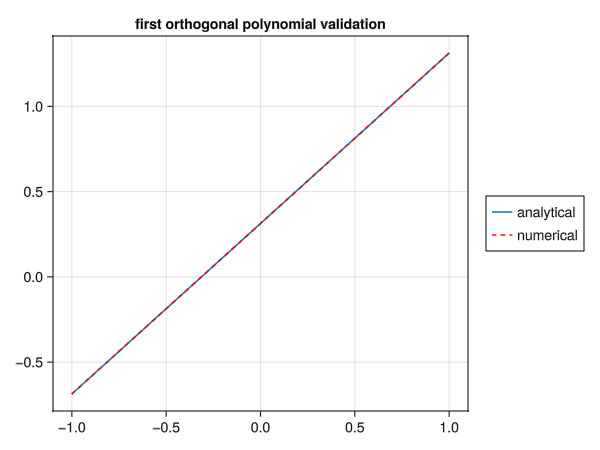
\includegraphics[width=0.7\textwidth,height=\textheight]{hw5_files/media/validationpione.png}
\caption{Validation of the stieltjes algorthim: Plot of numerical over
analytical solution of the first orthogonal polynomial}
\end{figure}

}

\caption{\label{fig-q1pa}}

\end{figure}%

\subsection{Part B}\label{part-b}

Veriy that the polynomial basis you obtained in part a is orthogonal,
i.e., that the matrix

\begin{equation}\tag{2}\label{polybasis}
\mathbb{E}\{P_k(\xi)P_j(\xi)\} = \int_{-1}^{1} P_k(x)P_j(x)dx
\end{equation} is diagonal.

\subsubsection{Solution}\label{solution-1}

Let us write a code that computes the Matrix and then plot the matrix
using a heatmap to check if it diagonal.

\begin{Shaded}
\begin{Highlighting}[]
\KeywordTok{function} \FunctionTok{isdiagonal}\NormalTok{(}\ConstantTok{π}\OperatorTok{::}\DataTypeTok{Vector\{Function\}}\NormalTok{, sup}\OperatorTok{::}\DataTypeTok{SVector\{2\}}\NormalTok{)}
\NormalTok{    A }\OperatorTok{=} \FunctionTok{Matrix}\DataTypeTok{\{Float64\}}\NormalTok{(}\ConstantTok{undef}\NormalTok{, }\FloatTok{7}\NormalTok{, }\FloatTok{7}\NormalTok{)}
    \ControlFlowTok{for}\NormalTok{ idx }\KeywordTok{in} \FunctionTok{CartesianIndices}\NormalTok{(A)}
\NormalTok{        (k, j) }\OperatorTok{=}\NormalTok{ idx.I}
\NormalTok{        ele }\OperatorTok{=} \FunctionTok{integ}\NormalTok{(x}\OperatorTok{{-}\textgreater{}} \ConstantTok{π}\NormalTok{[k}\OperatorTok{+}\FloatTok{1}\NormalTok{](x) }\OperatorTok{*} \ConstantTok{π}\NormalTok{[j}\OperatorTok{+}\FloatTok{1}\NormalTok{](x) }\OperatorTok{*} \FunctionTok{μ}\NormalTok{(x), sup)}
\NormalTok{        A[k, j] }\OperatorTok{=}\NormalTok{ ele }\OperatorTok{\textless{}} \FloatTok{1e{-}12}\NormalTok{ ? }\FloatTok{1e{-}8} \OperatorTok{:}\NormalTok{ ele}
    \ControlFlowTok{end}
\NormalTok{    fig }\OperatorTok{=} \FunctionTok{Figure}\NormalTok{()}
\NormalTok{    ax }\OperatorTok{=} \FunctionTok{Axis}\NormalTok{(fig[}\FloatTok{1}\NormalTok{, }\FloatTok{1}\NormalTok{], title }\OperatorTok{=} \StringTok{"heatmap of the diagona matrix"}\NormalTok{)}
    \FunctionTok{heatmap!}\NormalTok{(ax, }\FunctionTok{log10}\NormalTok{.(A))}
\NormalTok{    ax.yreversed}\OperatorTok{=}\ConstantTok{true}
    \FunctionTok{save}\NormalTok{(}\StringTok{"heatmapdiagonal.png"}\NormalTok{, fig)}
\KeywordTok{end}
\FunctionTok{isdiagonal}\NormalTok{(}\ConstantTok{π}\NormalTok{, sup)}
\end{Highlighting}
\end{Shaded}

\begin{figure}

\centering{

\begin{figure}
\centering
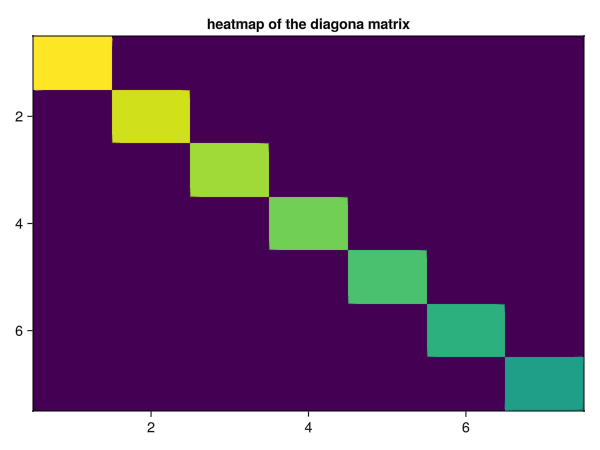
\includegraphics[width=0.7\textwidth,height=\textheight]{hw5_files/media/heatmapdiagonal.png}
\caption{Heatmap showing that the matrix of innerproducts with respect
to the weight function of all polynomials generated is diagonal.}
\end{figure}

}

\caption{\label{fig-q1pb}}

\end{figure}%

Clearly we can see that the matrix is diagonal and thus the polynomail
functions are orthogonal with respect to the weight function.

\subsection{Part C}\label{part-c}

Plot \(P_k(x)\) for \(k = 0, ..., 6\)

\subsubsection{Solution}\label{solution-2}

Let us define a code that plots all polynomials \(P_k(x)\) for
\(k = 0, ..., 6\)

\begin{Shaded}
\begin{Highlighting}[]
\KeywordTok{function} \FunctionTok{plotpolynomials}\NormalTok{(}\ConstantTok{π}\OperatorTok{::}\DataTypeTok{Vector\{Function\}}\NormalTok{)}
\NormalTok{    M }\OperatorTok{=} \FunctionTok{size}\NormalTok{(}\ConstantTok{π}\NormalTok{)[}\FloatTok{1}\NormalTok{]}
\NormalTok{    fig }\OperatorTok{=} \FunctionTok{Figure}\NormalTok{();}\FunctionTok{display}\NormalTok{(fig)}
\NormalTok{    ax }\OperatorTok{=} \FunctionTok{Axis}\NormalTok{(fig[}\FloatTok{1}\NormalTok{, }\FloatTok{1}\NormalTok{], title }\OperatorTok{=} \StringTok{"Plot of the set of orthogonal polynomials up to degree 6"}\NormalTok{)}
\NormalTok{    xs }\OperatorTok{=} \FunctionTok{LinRange}\NormalTok{(}\OperatorTok{{-}}\FloatTok{1.0}\NormalTok{, }\FloatTok{1.0}\NormalTok{, }\FloatTok{1000}\NormalTok{)}
    \ControlFlowTok{for}\NormalTok{ n }\KeywordTok{in} \FloatTok{1}\OperatorTok{:}\NormalTok{M}\OperatorTok{{-}}\FloatTok{1}
        \FunctionTok{lines!}\NormalTok{(ax, xs, }\ConstantTok{π}\NormalTok{[n}\OperatorTok{+}\FloatTok{1}\NormalTok{].(xs), label}\OperatorTok{=}\StringTok{"π\_}\SpecialCharTok{$}\NormalTok{(n}\OperatorTok{{-}}\FloatTok{1}\NormalTok{)}\StringTok{"}\NormalTok{)}
    \ControlFlowTok{end}
    \FunctionTok{Legend}\NormalTok{(fig[}\FloatTok{1}\NormalTok{, }\FloatTok{2}\NormalTok{], ax)}
    \FunctionTok{save}\NormalTok{(}\StringTok{"plotpolynomials.png"}\NormalTok{, fig)}
\KeywordTok{end}
\FunctionTok{plotpolynomials}\NormalTok{(}\ConstantTok{π}\NormalTok{)}
\end{Highlighting}
\end{Shaded}

\begin{figure}

\centering{

\begin{figure}
\centering
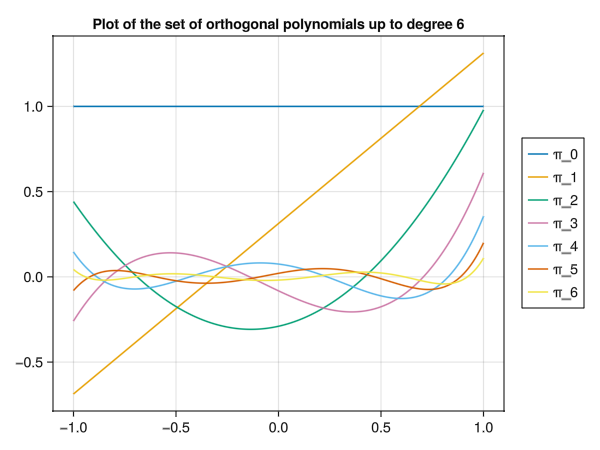
\includegraphics[width=0.7\textwidth,height=\textheight]{hw5_files/media/plotpolynomials.png}
\caption{Plot of polynomials within the support {[}-1, 1{]}}
\end{figure}

}

\caption{\label{fig-q1pc}}

\end{figure}%

\section{Question 2}\label{question-2}

Consider the following nonlinear fuction of the random variable
\(\xi(\omega)\) with PDF defined in \eqref{pxi}

\begin{equation}\tag{3}\label{eta}
\eta(\omega) = \frac{\xi(\omega) -1}{2 + 1\sin{(2\xi(\omega))}}
\end{equation}

\subsection{Part A}\label{part-a-1}

Compute the PDF of \(\eta\) using the relative frequency approach. To
this end, sample 50,000 realizations of \(\xi\) using the inverse CDF
approach applied to \eqref{pxi}, and use such samples to compute samples
of \(\eta(\omega)\).

\subsubsection{Solution}\label{solution-3}

The following code samples from \eqref{pxi} 50,000 times using the
inverse sampling method previously applied in Homework 1 and 2, then
applies the transformation \eqref{eta}, and finally plots the histogram
with 80 bins, normalized so that the PDF integrates to one over the
support.

\begin{Shaded}
\begin{Highlighting}[]
\FunctionTok{η}\NormalTok{(ξ) }\OperatorTok{=}\NormalTok{ (ξ }\OperatorTok{{-}} \FloatTok{1}\NormalTok{) }\OperatorTok{/}\NormalTok{ (}\FloatTok{2} \OperatorTok{+} \FunctionTok{sin}\NormalTok{(}\FloatTok{2}\OperatorTok{*}\NormalTok{ξ))}
\KeywordTok{function} \FunctionTok{question2a}\NormalTok{()}
\NormalTok{    r }\OperatorTok{=} \FunctionTok{LinRange}\NormalTok{(}\OperatorTok{{-}}\FloatTok{1}\NormalTok{, }\FloatTok{1}\NormalTok{, }\FloatTok{1000}\NormalTok{)}
\NormalTok{    fig }\OperatorTok{=} \FunctionTok{Figure}\NormalTok{();}\FunctionTok{display}\NormalTok{(fig)}
\NormalTok{    ax }\OperatorTok{=} \FunctionTok{Axis}\NormalTok{(fig[}\FloatTok{1}\NormalTok{, }\FloatTok{1}\NormalTok{],}
\NormalTok{        title }\OperatorTok{=} \StringTok{"PDF of η(ξ(ω))"}\NormalTok{)}
\NormalTok{    ys }\OperatorTok{=} \FunctionTok{cumsumtrap}\NormalTok{(μ, r)}
\NormalTok{    samples }\OperatorTok{=} \FunctionTok{Vector}\DataTypeTok{\{Float64\}}\NormalTok{(}\ConstantTok{undef}\NormalTok{, }\FloatTok{50000}\NormalTok{)}
    \ControlFlowTok{for}\NormalTok{ i }\KeywordTok{in} \FunctionTok{eachindex}\NormalTok{(samples)}
\NormalTok{        samples[i] }\OperatorTok{=} \FunctionTok{η}\NormalTok{(}\FunctionTok{sampleInverseCDF}\NormalTok{(}\FunctionTok{rand}\NormalTok{(), }\FunctionTok{hcat}\NormalTok{(ys, r)))}
    \ControlFlowTok{end}
    \FunctionTok{hist!}\NormalTok{(ax, samples, bins }\OperatorTok{=} \FloatTok{80}\NormalTok{, normalization }\OperatorTok{=} \OperatorTok{:}\NormalTok{pdf)}
    \FunctionTok{save}\NormalTok{(}\StringTok{"question2a.png"}\NormalTok{, fig)}
\NormalTok{    samples}
\KeywordTok{end}
\NormalTok{samples }\OperatorTok{=} \FunctionTok{question2a}\NormalTok{();}
\end{Highlighting}
\end{Shaded}

\begin{figure}

\centering{

\begin{figure}
\centering
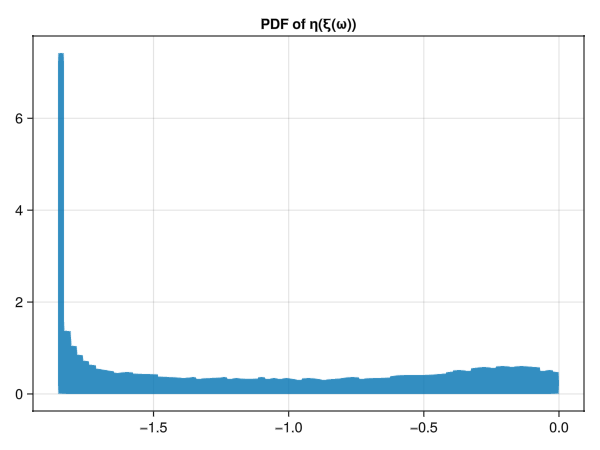
\includegraphics[width=0.7\textwidth,height=\textheight]{hw5_files/media/question2a.png}
\caption{PDF of \(\eta(\xi(\omega))\) by sampling 50,000 times via
inverse CDF approach and applying the transformation \eqref{eta}}
\end{figure}

}

\caption{\label{fig-q2pa}}

\end{figure}%

\subsection{Part B}\label{part-b-1}

Show numerically that the gPC expansion \footnote{Note that
  \(\mathbb{E}\{\eta(\xi(\omega))P_k(\xi(\omega))\}\) can be computed
  with MC, or with quadrature as
  \begin{equation}\tag{4}\label{four}\mathbb{E}\{\eta(\xi(\omega))P_k(\xi(\omega))\}= \int_{-1}^{1}\frac{x - 1}{2 + 1 \sin(2x)}P_k(x)P_\xi(x)dx\end{equation}}

\begin{equation}\tag{5}\label{gpc}
\eta_M(\omega) = \sum_{k=0}^{M}a_k P_k(\xi(\omega)), \quad a_k = \frac{\mathbb{E}\{\eta(\xi(\omega))P_k(\xi(\omega))\}}{\mathbb{E}\{P_k^2(\xi(\omega))\}}
\end{equation}

converges to \(\eta(\omega)\) in distribution as \(M\) increases. To
this end, plot the PDF of the random variables \(\eta_M(\xi(\omega))\)
for \(M = 1, 2, 4, 6\) using method of relative frequencies and compare
such PDF's with the PDF of \(\eta\) you computed in part a.

\subsubsection{Solution}\label{solution-4}

\begin{Shaded}
\begin{Highlighting}[]
\KeywordTok{function} \FunctionTok{question2b}\NormalTok{(πn}\OperatorTok{::}\DataTypeTok{Vector\{Function\}}\NormalTok{)}
\NormalTok{    a }\OperatorTok{=} \FunctionTok{Vector}\DataTypeTok{\{Float64\}}\NormalTok{(}\ConstantTok{undef}\NormalTok{, }\FloatTok{7}\NormalTok{)}
\NormalTok{    colors }\OperatorTok{=} \DataTypeTok{Symbol}\NormalTok{[}\OperatorTok{:}\NormalTok{red, }\OperatorTok{:}\NormalTok{green, }\OperatorTok{:}\NormalTok{blue, }\OperatorTok{:}\NormalTok{yellow, }\OperatorTok{:}\NormalTok{orange, }\OperatorTok{:}\NormalTok{purple]}
    \CommentTok{\# calculate coefficients}
    \ControlFlowTok{for}\NormalTok{ k }\KeywordTok{in} \FunctionTok{eachindex}\NormalTok{(a)}
\NormalTok{        a[k] }\OperatorTok{=} \FunctionTok{integ}\NormalTok{(x }\OperatorTok{{-}\textgreater{}} \FunctionTok{η}\NormalTok{(x) }\OperatorTok{*}\NormalTok{ πn[k}\OperatorTok{+}\FloatTok{1}\NormalTok{](x) }\OperatorTok{*} \FunctionTok{μ}\NormalTok{(x), sup) }\OperatorTok{/} \FunctionTok{integ}\NormalTok{(x }\OperatorTok{{-}\textgreater{}}\NormalTok{ πn[k}\OperatorTok{+}\FloatTok{1}\NormalTok{](x) }\OperatorTok{*}\NormalTok{ πn[k}\OperatorTok{+}\FloatTok{1}\NormalTok{](x) }\OperatorTok{*} \FunctionTok{μ}\NormalTok{(x), sup)}
    \ControlFlowTok{end}
    
\NormalTok{    fig }\OperatorTok{=} \FunctionTok{Figure}\NormalTok{();}\FunctionTok{display}\NormalTok{(fig)}
\NormalTok{    ax }\OperatorTok{=} \FunctionTok{Axis}\NormalTok{(fig[}\FloatTok{1}\NormalTok{, }\FloatTok{1}\NormalTok{], title}\OperatorTok{=}\StringTok{"densities of ηM(ξ(ω)) for M = \{1, 2, 4, 6\}"}\NormalTok{)}
\NormalTok{    r }\OperatorTok{=} \FunctionTok{LinRange}\NormalTok{(}\OperatorTok{{-}}\FloatTok{1}\NormalTok{, }\FloatTok{1}\NormalTok{, }\FloatTok{1000}\NormalTok{)}
\NormalTok{    ys }\OperatorTok{=} \FunctionTok{hcat}\NormalTok{(}\FunctionTok{cumsumtrap}\NormalTok{(μ, r), r)}
    \ControlFlowTok{for}\NormalTok{ M }\KeywordTok{in} \FunctionTok{SVector}\DataTypeTok{\{4\}}\NormalTok{(}\FloatTok{1}\NormalTok{, }\FloatTok{2}\NormalTok{, }\FloatTok{4}\NormalTok{, }\FloatTok{6}\NormalTok{)}
\NormalTok{        ηM\_samples }\OperatorTok{=} \FunctionTok{Vector}\DataTypeTok{\{Float64\}}\NormalTok{(}\ConstantTok{undef}\NormalTok{, }\FloatTok{50000}\NormalTok{)}
        \ControlFlowTok{for}\NormalTok{ l }\KeywordTok{in} \FunctionTok{eachindex}\NormalTok{(ηM\_samples)}
\NormalTok{            η\_sum }\OperatorTok{=} \FloatTok{0.0}
\NormalTok{            ξ }\OperatorTok{=} \FunctionTok{sampleInverseCDF}\NormalTok{(}\FunctionTok{rand}\NormalTok{(), ys)}
            \ControlFlowTok{for}\NormalTok{ k }\KeywordTok{in} \FloatTok{1}\OperatorTok{:}\NormalTok{M}\OperatorTok{+}\FloatTok{1}
\NormalTok{                η\_sum}\OperatorTok{+=}\NormalTok{a[k]}\OperatorTok{*}\NormalTok{πn[k}\OperatorTok{+}\FloatTok{1}\NormalTok{](ξ)}
            \ControlFlowTok{end}
\NormalTok{            ηM\_samples[l] }\OperatorTok{=}\NormalTok{ η\_sum}
        \ControlFlowTok{end}
        \FunctionTok{density!}\NormalTok{(ax, ηM\_samples, color }\OperatorTok{=}\NormalTok{ (colors[M], }\FloatTok{0.3}\NormalTok{), label }\OperatorTok{=} \StringTok{"M = }\SpecialCharTok{$}\NormalTok{M}\StringTok{"}\NormalTok{, strokecolor }\OperatorTok{=}\NormalTok{ colors[M], strokewidth }\OperatorTok{=} \FloatTok{3}\NormalTok{, strokearound }\OperatorTok{=} \ConstantTok{true}\NormalTok{) }
    \ControlFlowTok{end}
    \FunctionTok{Legend}\NormalTok{(fig[}\FloatTok{1}\NormalTok{, }\FloatTok{2}\NormalTok{], ax)}
    \FunctionTok{save}\NormalTok{(}\StringTok{"question2b.png"}\NormalTok{, fig)}
\KeywordTok{end}
\FunctionTok{question2b}\NormalTok{(}\ConstantTok{π}\NormalTok{);}
\end{Highlighting}
\end{Shaded}

\begin{figure}

\centering{

\begin{figure}
\centering
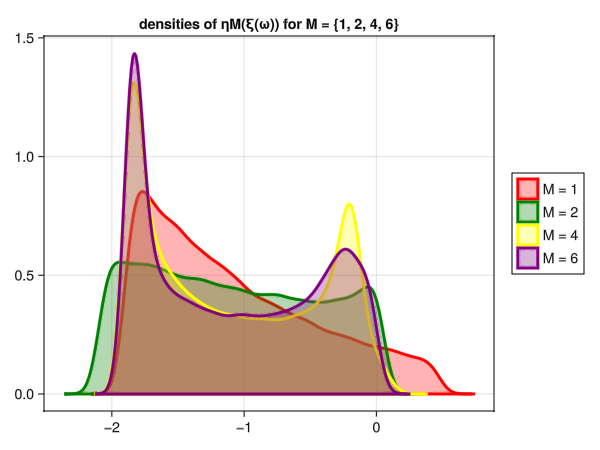
\includegraphics[width=0.7\textwidth,height=\textheight]{hw5_files/media/question2b.png}
\caption{The PDF ploted using Kernel Density Estimation for values M =
\{1, 2, 4, 6\}}
\end{figure}

}

\caption{\label{fig-q2pb}}

\end{figure}%

As we can see, the PDF of the random variable \(\eta_M(\omega)\)
converges to the PDF of \(\eta(\omega)\) as M increases.

\subsection{Part C}\label{part-c-1}

Compute the mean and variance of \(\eta_6\) and compare it with the mean
and variance of \(\eta\). Note that such means and variances can be
computed in multiple ways, e.g., by using MC, or by approximating the
integral defining the moments of the random variable \(\eta\) using
quadrature, e.g., via the trapezoidal rule applied to the integral

\begin{equation}\tag{6}\label{quadr}
\mathbb{E}\{\eta^k\} = \int_{-1}^{1} \left(\frac{x-1}{2+\sin(2x)}\right)^k p_{\xi}(x)dx
\end{equation}

\subsubsection{Solution}\label{solution-5}

Let us find the mean and variance of \(\eta\) and \(\eta_6\) by
generating 1000 samples of size 1000 and taking the average of the mean
and variance for each sample.

\begin{Shaded}
\begin{Highlighting}[]
\KeywordTok{function} \FunctionTok{question2c}\NormalTok{()}
\NormalTok{    r }\OperatorTok{=} \FunctionTok{LinRange}\NormalTok{(}\OperatorTok{{-}}\FloatTok{1}\NormalTok{, }\FloatTok{1}\NormalTok{, }\FloatTok{1000}\NormalTok{)}
\NormalTok{    ys }\OperatorTok{=} \FunctionTok{hcat}\NormalTok{(}\FunctionTok{cumsumtrap}\NormalTok{(μ, r), r)}
\NormalTok{    η\_samples }\OperatorTok{=} \FunctionTok{Vector}\DataTypeTok{\{Float64\}}\NormalTok{(}\ConstantTok{undef}\NormalTok{, }\FloatTok{50000}\NormalTok{)}
    \ControlFlowTok{for}\NormalTok{ i }\KeywordTok{in} \FunctionTok{eachindex}\NormalTok{(η\_samples)}
\NormalTok{        η\_samples[i] }\OperatorTok{=} \FunctionTok{η}\NormalTok{(}\FunctionTok{sampleInverseCDF}\NormalTok{(}\FunctionTok{rand}\NormalTok{(), ys))}
    \ControlFlowTok{end}
\NormalTok{    a }\OperatorTok{=} \FunctionTok{Vector}\DataTypeTok{\{Float64\}}\NormalTok{(}\ConstantTok{undef}\NormalTok{, }\FloatTok{7}\NormalTok{)}
    \ControlFlowTok{for}\NormalTok{ k }\KeywordTok{in} \FunctionTok{eachindex}\NormalTok{(a)}
\NormalTok{        a[k] }\OperatorTok{=} \FunctionTok{integ}\NormalTok{(x }\OperatorTok{{-}\textgreater{}} \FunctionTok{η}\NormalTok{(x) }\OperatorTok{*}\NormalTok{ πn[k}\OperatorTok{+}\FloatTok{1}\NormalTok{](x) }\OperatorTok{*} \FunctionTok{μ}\NormalTok{(x), sup) }\OperatorTok{/} \FunctionTok{integ}\NormalTok{(x }\OperatorTok{{-}\textgreater{}}\NormalTok{ πn[k}\OperatorTok{+}\FloatTok{1}\NormalTok{](x) }\OperatorTok{*}\NormalTok{ πn[k}\OperatorTok{+}\FloatTok{1}\NormalTok{](x) }\OperatorTok{*} \FunctionTok{μ}\NormalTok{(x), sup)}
    \ControlFlowTok{end}
\NormalTok{    η}\FloatTok{6}\NormalTok{\_samples }\OperatorTok{=} \FunctionTok{Vector}\DataTypeTok{\{Float64\}}\NormalTok{(}\ConstantTok{undef}\NormalTok{, }\FloatTok{50000}\NormalTok{)}
    \ControlFlowTok{for}\NormalTok{ l }\KeywordTok{in} \FunctionTok{eachindex}\NormalTok{(η}\FloatTok{6}\NormalTok{\_samples)}
\NormalTok{        η\_sum }\OperatorTok{=} \FloatTok{0.0}
\NormalTok{        ξ }\OperatorTok{=} \FunctionTok{sampleInverseCDF}\NormalTok{(}\FunctionTok{rand}\NormalTok{(), ys)}
        \ControlFlowTok{for}\NormalTok{ k }\KeywordTok{in} \FunctionTok{eachindex}\NormalTok{(a)}
\NormalTok{            η\_sum}\OperatorTok{+=}\NormalTok{a[k]}\OperatorTok{*}\NormalTok{πn[k}\OperatorTok{+}\FloatTok{1}\NormalTok{](ξ)}
        \ControlFlowTok{end}
\NormalTok{        η}\FloatTok{6}\NormalTok{\_samples[l] }\OperatorTok{=}\NormalTok{ η\_sum}
    \ControlFlowTok{end}

\NormalTok{    means }\OperatorTok{=} \FunctionTok{Vector}\DataTypeTok{\{Float64\}}\NormalTok{(}\ConstantTok{undef}\NormalTok{, }\FloatTok{1000}\NormalTok{)}
\NormalTok{    variances }\OperatorTok{=} \FunctionTok{Vector}\DataTypeTok{\{Float64\}}\NormalTok{(}\ConstantTok{undef}\NormalTok{, }\FloatTok{1000}\NormalTok{)}
    \ControlFlowTok{for}\NormalTok{ i }\KeywordTok{in} \FunctionTok{eachindex}\NormalTok{(means)}
\NormalTok{        sample }\OperatorTok{=} \FunctionTok{rand}\NormalTok{(η\_samples, }\FloatTok{1000}\NormalTok{)}
\NormalTok{        means[i] }\OperatorTok{=} \FunctionTok{mean}\NormalTok{(sample)}
\NormalTok{        variances[i] }\OperatorTok{=} \FunctionTok{var}\NormalTok{(sample)}
    \ControlFlowTok{end}
\NormalTok{    η\_mean }\OperatorTok{=} \FunctionTok{mean}\NormalTok{(means)}
\NormalTok{    η\_var }\OperatorTok{=} \FunctionTok{mean}\NormalTok{(variances)}

\NormalTok{    means }\OperatorTok{=} \FunctionTok{Vector}\DataTypeTok{\{Float64\}}\NormalTok{(}\ConstantTok{undef}\NormalTok{, }\FloatTok{1000}\NormalTok{)}
\NormalTok{    variances }\OperatorTok{=} \FunctionTok{Vector}\DataTypeTok{\{Float64\}}\NormalTok{(}\ConstantTok{undef}\NormalTok{, }\FloatTok{1000}\NormalTok{)}
    \ControlFlowTok{for}\NormalTok{ i }\KeywordTok{in} \FunctionTok{eachindex}\NormalTok{(means)}
\NormalTok{        sample }\OperatorTok{=} \FunctionTok{rand}\NormalTok{(η}\FloatTok{6}\NormalTok{\_samples, }\FloatTok{1000}\NormalTok{)}
\NormalTok{        means[i] }\OperatorTok{=} \FunctionTok{mean}\NormalTok{(sample)}
\NormalTok{        variances[i] }\OperatorTok{=} \FunctionTok{var}\NormalTok{(sample)}
    \ControlFlowTok{end}
\NormalTok{    η}\FloatTok{6}\NormalTok{\_mean }\OperatorTok{=} \FunctionTok{mean}\NormalTok{(means)}
\NormalTok{    η}\FloatTok{6}\NormalTok{\_var }\OperatorTok{=} \FunctionTok{mean}\NormalTok{(variances)}
\NormalTok{    fig }\OperatorTok{=} \FunctionTok{Figure}\NormalTok{();}\FunctionTok{display}\NormalTok{(fig)}
\NormalTok{    ax }\OperatorTok{=} \FunctionTok{Axis}\NormalTok{(fig[}\FloatTok{1}\NormalTok{, }\FloatTok{1}\NormalTok{],}
\NormalTok{        xticks }\OperatorTok{=}\NormalTok{ (}\FloatTok{1}\OperatorTok{:}\FloatTok{2}\NormalTok{, [}\StringTok{"η"}\NormalTok{, }\StringTok{"η₆"}\NormalTok{]),}
\NormalTok{    title }\OperatorTok{=} \StringTok{"mean and variance for η and η\_6"}\NormalTok{)}
    \FunctionTok{barplot!}\NormalTok{(ax, [}\FloatTok{1}\NormalTok{, }\FloatTok{1}\NormalTok{, }\FloatTok{2}\NormalTok{, }\FloatTok{2}\NormalTok{], [η\_mean, η\_var, η}\FloatTok{6}\NormalTok{\_mean, η}\FloatTok{6}\NormalTok{\_var],}
\NormalTok{        dodge }\OperatorTok{=}\NormalTok{ [}\FloatTok{1}\NormalTok{, }\FloatTok{2}\NormalTok{, }\FloatTok{1}\NormalTok{, }\FloatTok{2}\NormalTok{],}
\NormalTok{        color }\OperatorTok{=}\NormalTok{ [}\FloatTok{1}\NormalTok{, }\FloatTok{2}\NormalTok{, }\FloatTok{1}\NormalTok{, }\FloatTok{2}\NormalTok{])}
    \FunctionTok{save}\NormalTok{(}\StringTok{"question2c.png"}\NormalTok{, fig)}
\KeywordTok{end}
\FunctionTok{question2c}\NormalTok{();}
\end{Highlighting}
\end{Shaded}

\begin{figure}

\centering{

\begin{figure}
\centering
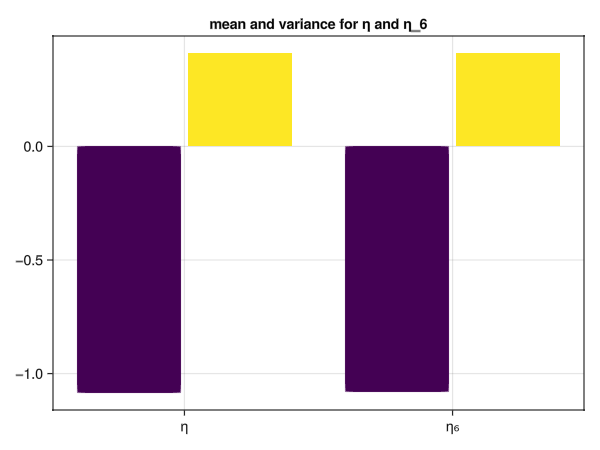
\includegraphics[width=0.7\textwidth,height=\textheight]{hw5_files/media/question2c.png}
\caption{Barplot of the bootstrap mean and variance from MC for \(\eta\)
and \(\eta_6\)}
\end{figure}

}

\caption{\label{fig-q2pc}}

\end{figure}%

From the plot we can see the the sample meand and variance for both are
almost identical.

\section{Question 3}\label{question-3}

Compute the solution of the following random initial value problem

\begin{equation}\tag{7}\label{randomivp}
\begin{cases}
    \frac{x}{t} &= -xi(\omega)x + \cos(4t) \\
    x(0) &= 1
\end{cases}
\end{equation}

using the stocastic Galerkin method with the gPC basis you obtained in
question 1. In particular, use the following gPC expansion of degree 6
for the solution of \eqref{randomivp}.

\begin{equation}\tag{8}\label{eight}
x(t;\omega) = \sum_{k=0}^6 \hat{x}_k(t)P_k(\xi(\omega))
\end{equation}

where the gPC modes \(\hat{x}_k(t)\) are to be determined from
\eqref{randomivp}.

\subsection{Part A}\label{part-a-2}

Compute the mean and the variance of \eqref{eight} fot \(t \in [0, 3]\).

\subsubsection{Solution}\label{solution-6}

\subsection{Part B}\label{part-b-2}

Compute the PDF of \eqref{eight} at times \(\{0.5, 1, 2, 3\}\) (use
relative frequencies).

Note: you can debug your gPC results by either computing the analytic
solution of \eqref{randomivp} and then computing moments/PDFs of such
solutions as a function of \(t\), or by randomly sampling many solution
paths of \eqref{randomivp} and then computing ensemble averages.

\subsubsection{Solution}\label{solution-7}

\section{Appendix}\label{appendix}

\subsection{Figures}\label{figures}

\begin{figure}

\centering{

\begin{figure}
\centering
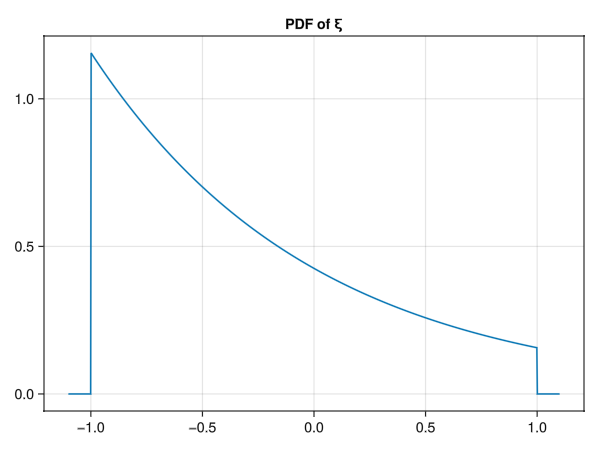
\includegraphics[width=0.5\textwidth,height=\textheight]{hw5_files/media/PDFone.png}
\caption{The PDF of \(\xi\)}
\end{figure}

}

\caption{\label{fig-pdfxi}}

\end{figure}%




\end{document}
